\documentclass[10pt,a4paper]{article}

\usepackage[margin=0.5cm]{geometry}
\usepackage{multicol}
\usepackage{amsmath, amssymb}
\usepackage{tcolorbox}
\usepackage{enumitem}
\usepackage{makecell}
\usepackage{tabularx}
\usepackage{tikz}
\usepackage{pgfplots}
\pgfplotsset{compat=1.18} % latest stable

\usepackage{tikz}
\usepackage[utf8]{inputenc}
\usepackage[T1]{fontenc}
\usetikzlibrary{arrows.meta}

% compact lists
\setlist{nosep}

% compact sections
\setlength{\parindent}{0pt}
\setlength{\parskip}{0pt}

\begin{document}

\begin{center}
  \bfseries\Huge Questionario Socrative
\end{center}
\vspace{20pt}

\begin{multicols}{2}
    1. ¿Qué tipo de modulación digital representa la constelación mostrada en la figura adjunta?
    
    \begin{enumerate}[label=\alph*]
        \item Modulación ASK multinivel.
        \item Modulación PSK multinivel.
        \item \textbf{Modulación combinada de amplitud y fase.}
        \item Modulación FSK multinivel.
    \end{enumerate}
    \columnbreak
    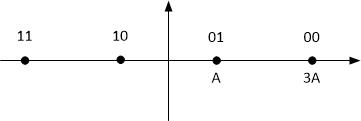
\includegraphics[width=0.5\textwidth]{1.jpeg}
\end{multicols}
\textbf{Explicación}

Esta modulación combina 2 amplitudes (A y 3A, pues la constelación se supone simétrica) y 2 fases (0 y 180º), por lo que se trata de una modulación combinada de amplitud y fase.

\vspace{15pt} \hrule

\begin{multicols}{2}
    {
        2. Un transmisor hace uso de la modulación representada en la figura adjunta. Suponiendo que los dígitos 0 y 1 tienen la misma probabilidad (codificación de fuente óptima), ¿qué afirmación es correcta acerca de la potencia media transmitida?
        \begin{enumerate}[label=\alph*]
            \item La potencia media transmitida es 10 veces mayor que la potencia media con la que se transmiten los símbolos 01 y 10.
            \item \textbf{La potencia media transmitida es 5 veces mayor que la potencia media con la que se transmiten los símbolos 01 y 10.}
            \item La potencia media transmitida es 2.5 veces mayor que la potencia media con la que se transmiten los símbolos 01 y 10.
            \item La potencia media transmitida es 2 veces mayor que la potencia media con la que se transmiten los símbolos 01 y 10.
        \end{enumerate}
    }
    \columnbreak
    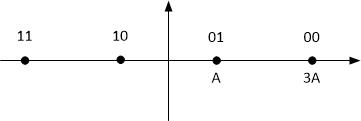
\includegraphics[width=0.5\textwidth]{1.jpeg}
\end{multicols}
\textbf{Explicación}

La potencia media de una señal sinusoidal es su amplitud al cuadrado dividido por 2. Por lo tanto, la potencia media con que se transmiten los símbolos 01 y 10 es $\frac{A^2}{2}$ y la potencia media con que se transmiten los símbolos 00 y 11 es $\frac{(3A)^2}{2} = \frac{9A^2}{2}$.

Como los dígitos 0 y 1 son equiprobables, también lo son los 4 símbolos, por lo que la potencia media global es $\frac{2\frac{A^2}{2} + \frac{9A^2}{2}}{4} = \frac{10A^2}{4} = 5\frac{A^2}{2}$.
Este resultado corresponde a 5 veces la potencia media con la que se transmiten los símbolos 01 y 10.

\vspace{15pt} \hrule
\vspace{15pt}

3. La potencia media disipada por un pulso de voltaje rectangular de duración $\tau$ segundos y amplitud $A$ voltios, sobre una resistencia equivalente de R ohmios viene dada por la siguiente expresión:
\begin{enumerate}[label=\alph*]
    \item $A^2/(\tau R) \mathrm{W}$
    \item $A^2/(2\tau R) \mathrm{dBW}$
    \item $\mathbf{A^2/R \mathrm{\textbf{W}}}$
    \item $A^2/(2\tau) \mathrm{dBW}$
\end{enumerate}
\textbf{Explicación}

La potencia instantánea es $\frac{A^2}{R}$ durante el intervalo de tiempo de duración de la señal, que es $\tau$. Al aplicar la fórmula de cálculo de la potencia media de una señal de duración finita, el resultado es  
$\frac{1}{\tau}\int_\tau{\frac{A^2}{R}dt} = \frac{A^2}{R} \mathrm{W}$ (watios porque la amplitud y el tiempo están exprasados en unidades internacionales, es decir, voltios y segundos respectivamente).

\vspace{15pt} \hrule
\pagebreak

\begin{multicols}{2}
    {
        4. ¿Cuánto vale la ganancia del amplificador ideal de la figura, suponiendo que trabaja en la zona lineal?
        \begin{enumerate}[label=\alph*]
            \item Unos 17 dBW.
            \item Unos 17 dBm.
            \item 100 dB.
            \item \textbf{Unos 17 dB.}
        \end{enumerate}
    }
    \columnbreak
    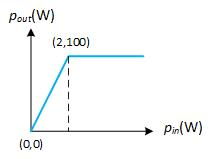
\includegraphics[width=0.5\textwidth]{2.jpeg}
\end{multicols}
\textbf{Explicación}

En la zona lineal, la recta que relaciona potencia de salida con potencia de entrada es $P_{out} = 50P_{in}, 0 \leq P_{in} \leq 2 \mathrm{W}$.
Por tanto, la ganancia de este amplificador será $10\log_{10}{\frac{P_{out}}{P_{in}}} = 10\log_{10}{\frac{5P_{in}}{P_{in}}} = 10\log_{10}{5} \approx 17$ dB

\vspace{15pt} \hrule

\begin{multicols}{2}
    {
        5. La figura muestra el espectro de potencia de una señal. ¿Cuál de las siguientes afirmaciones es correcta?
        \begin{enumerate}[label=\alph*]
            \item La señal no es periódica.
            \item Es una señal periódica cuya frecuencia fundamental es 150 KHz.
            \item Es una señal periódica cuya frecuencia fundamental es 25 KHz.
            \item \textbf{Es una señal periódica cuyo período vale 20 microsegundos.}
        \end{enumerate}
    }
    \columnbreak
    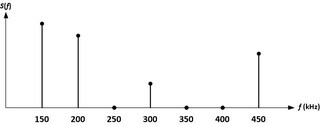
\includegraphics[width=0.5\textwidth]{3.jpeg}
\end{multicols}
\textbf{Explicación}

Al tratarse de un espectro discreto, la señal es periódica.  La frecuencia fundamental de una señal periódica es el máximo común divisor de las frecuencias contenidas en dicha señal.

En este caso, las frecuencias contenidas (aquellas cuya barra no es nula) son 150, 200, 300 y 450 (todas en KHz), cuyo máximo común divisor es 50. Por tanto, la frecuencia fundamental es 50 KHz.

Como el período de la señal periódica es la inversa de su frecuencia fundamental, en este caso vale 0.02 ms, es decir, 20 microsegundos.

\vspace{15pt} \hrule \vspace{15pt}

6. La señal $5\sin(500\pi t + \frac{\pi}{2})$, donde $t$ se expresa en ms, se propaga a través de un medio de transmisión guiado que atenúa a razón de 1.5 dB/Km, y cuya velocidad de propagación es de 250000 Km/s. Señalar la afirmación correcta acerca de dicha señal:

\begin{enumerate}[label=\alph*]
    \item Su longitud de onda es de 500 m.
    \item Su período es de 2 microsegundos.
    \item \textbf{Su amplitud al haber recorrido 4 Km es 2.5.}
    \item Ninguna de las anteriores afirmaciones es correcta.
\end{enumerate}
\textbf{Explicación}

La frecuencia de esta señal sinusoidal es de 250 KHz (250 porque la expresión estándar de una señal sinusoidal es $A \sin(2\pi f t + \phi)$, con lo que el valor 500 debe corresponder a $2f$, y KHz porque se dice que $t$ está expresado en ms). Por tanto, la longitud de onda de esta señal es $\lambda = \frac{v_{prop}}{f} = \frac{250000}{250 \cdot 10^3} = 1$ Km.

Su período vale $T = \frac{1}{f} = \frac{1}{250} = 0.004$ ms, es decir, 4 microsegundos.

Si el medio guiado introduce una atenuación de 1.5 dB/Km, al haber recorrido 4 Km, la señal se habrá atenuado 6 dB. Esto corresponde a una caída de potencia de valor 4, pues $10\log_{10}4 \approx 6$.

Como la potencia es proporcional a la amplitud al cuadrado, dividir la potencia por 4 supone dividir la amplitud por 2, por lo que la amplitud resultante al cabo de 4 Km es la mitad de la amplitud de salida, es decir, la mitad de 5, que es 2.5.

\vspace{15pt} \hrule
\pagebreak

\begin{multicols}{2}
    {
        7. La figura muestra la conexión entre un transmisor y un receptor a través de una cascada de amplificadores. ¿Cuál debe ser la ganancia mínima de estos amplificadores (se suponen todos iguales), si la potencia de salida del transmisor es igual a 1 W y la sensibilidad del receptor es de 2.5 mW?
        \begin{enumerate}[label=\alph*]
            \item \textbf{18.5 dB.}
            \item 26.0 dB.
            \item 33.5 dB.
            \item Ninguna de las anteriores.
        \end{enumerate}
    }
    \columnbreak
    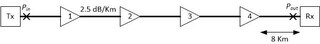
\includegraphics[width=0.5\textwidth]{4.jpeg}
\end{multicols}
\textbf{Explicación}

Trabajando con unidades logarítmicas, el problama se plantea como una inecuación basada en sumas y restas.

Teniendo en cuenta que la sensibilidad de un receptor es la potencia media mínima que tiene que haber a su entrada para que dicho receptor pueda detectar la presencia de la señal, la inecuación que se plantea, es la siguiente, donde $G$ (ganancia en dB de los 4 amplificadores, pues son todos iguales) es la incógnita: 
$0 - 5 \cdot 2.5 \cdot 8 + 4 \geq 10\log_{10}{0.0025}$, es decir, $-100 + 4 \geq - 26$ , de donde se obtiene que $G \geq 18.5$ dB.

Nótese que se ha trabajado en dBW, y por ello la potencia transmitida se ha expresado como 0 dBW, y los milivatios de sensibilidad se han pasado a W antes de convertirlos a dBW.

\vspace{15pt} \hrule \vspace{15pt}

8. Una fibra óptica monomodo que trabaja en la banda de 1550 nm presenta una atenuación de 0.5 dB/Km. ¿Qué distancia tiene que haber recorrido la señal para que su potencia se vea dividida por 16?

\begin{enumerate}[label=\alph*]
    \item \textbf{Unos 24 Km.}
    \item Unos 12 Km.
    \item Unos 48 Km.
    \item Ninguna de las anteriores.
\end{enumerate}
\textbf{Explicación}

Si la potencia se divide por 16, significa que la señal ha experimentado una caída de $10\log_{10}{16} \approx 12$ dB, para lo cual la señal tiene que haber recorrido 24 Km.

\vspace{15pt} \hrule \vspace{15pt}

9. El retardo de propagación de ida y vuelta en un enlace vía satélite geoestacionario vale, aproximadamente:

\begin{enumerate}[label=\alph*]
    \item 120 ms.
    \item 240 ms.
    \item 360 ms.
    \item \textbf{480 ms.}
\end{enumerate}
\textbf{Explicación}

Redondeando la distancia entre la Tierra y un satélite geoestacionario a 36000 Km, el retardo de propagación de subida o bajada vale $\frac{36000}{300000} = 0.12$s, que son 120 ms.

En un enlace vía satélite, el satélite es un intermediario entre dos estaciones terrenas, por lo que el retardo de propagación será el equivalente a subir y bajar, es decir, 240 ms. Por lo tanto, el retardo de propagación de ida y vuelta será de 480 ms.

\vspace{15pt} \hrule \vspace{15pt}

10. Una señal 8B6T transporta información a 300 Kbps. ¿Cuánto vale el ancho de banda mínimo del canal?

\begin{enumerate}[label=\alph*]
    \item 100 KHz.
    \item 150 KHz.
    \item \textbf{112.5 KHz.}
    \item 225 KHz.
\end{enumerate}
\textbf{Explicación}

Necesitamos calcular la velocidad de señalización: $R_s = \frac{R}{r} = \frac{300}{\frac{8}{6}} = 225$ KBaud. Según el criterio de Nyquist, el ancho de banda mínimo del canal es  
$\frac{R_s}{2} = \frac{225}{2} = 112.5$ KHz.

\end{document}